% !TeX encoding = UTF-8
% !TeX program = pdflatex
% !TeX spellcheck = it_IT
\documentclass[a4paper, twocolumn]{article}

\usepackage[utf8]{inputenc}
\usepackage[T1]{fontenc}
\usepackage[italian]{babel}
\usepackage[a4paper, left=2cm, right=2cm, top=2.6cm, bottom=2.6cm]{geometry} % Required to change the paper margin (the defaults are too large, values adjusted heuristically).
\usepackage{csquotes} % Required by babel for better quotes.
\usepackage{graphicx} % Required for inserting images.
\usepackage[style=alphabetic, sorting=ynt, maxnames=2]{biblatex} % Required for the bibliography.
\usepackage{subcaption} % To have subfigures and subcaptions in one figure.
\usepackage{hyperref} % For links, urls ettc.
\usepackage{amsfonts} % Required for math formulas.
\usepackage{mathtools} % Idem as above.
\usepackage[italian, noabbrev]{cleveref} % For automatic references label.
\usepackage{numprint} % To print numbers with separators and exponent.

% Add bibliography sources.
\addbibresource{references.bib}

\newcommand{\thetitle}{Apprendimento per rinforzo multi-agente per la distribuzione del carico in servizi di edge computing FaaS}
\newcommand{\theauthor}{Emanuele Petriglia}
\newcommand{\theversion}{16 Ottobre 2024}

\title{\thetitle}
\author{\theauthor}
\date{\theversion}

% Hyperref configuration.
\hypersetup{
  pdftitle     = {\thetitle},
  pdfauthor    = {\theauthor},
  colorlinks   = true,
  urlcolor     = black,
  linkcolor    = black,
  citecolor    = black
}

% Compacted bibliography.
% Thanks to: https://tex.stackexchange.com/a/170312
\DeclareBibliographyAlias{article}{std}
\DeclareBibliographyAlias{book}{std}
\DeclareBibliographyAlias{booklet}{std}
\DeclareBibliographyAlias{collection}{std}
\DeclareBibliographyAlias{inbook}{std}
\DeclareBibliographyAlias{incollection}{std}
\DeclareBibliographyAlias{inproceedings}{std}
\DeclareBibliographyAlias{manual}{std}
\DeclareBibliographyAlias{misc}{std}
\DeclareBibliographyAlias{online}{std}
\DeclareBibliographyAlias{patent}{std}
\DeclareBibliographyAlias{periodical}{std}
\DeclareBibliographyAlias{proceedings}{std}
\DeclareBibliographyAlias{report}{std}
\DeclareBibliographyAlias{thesis}{std}
\DeclareBibliographyAlias{unpublished}{std}
\DeclareBibliographyAlias{*}{std}

\DeclareBibliographyDriver{std}{%
  \usebibmacro{bibindex}%
  \usebibmacro{begentry}%
  \usebibmacro{author/editor+others/translator+others}%
  \setunit{\labelnamepunct}\newblock
  \usebibmacro{title}%
  \newunit\newblock
  \usebibmacro{date}%
  \newunit\newblock
  \usebibmacro{finentry}}

% Set the distance between columns.
\setlength{\columnsep}{25pt}

\begin{document}

% Title section.
\twocolumn[{%
    \centering

    {\LARGE \textbf{\thetitle}}

    \vspace{2mm}

    \large

    {\theauthor} -- 888435

    \begin{flushleft}
        \noindent
        {\textbf{Relatore:} Prof. Michele Ciavotta } \\
    
        \noindent
        {\textbf{Correlatrice:} Dott.ssa Federica Filippini}
    \end{flushleft}

    {\textbf{Sintesi Tesi di Laurea Magistrale} -- \theversion}

    \vspace{1cm} % Add space between title and content.
}]

\section{Introduzione}
\label{sec:introduction}

Negli ultimi anni, il mondo dell'Internet of Things (IoT) ha vissuto uno sviluppo senza precedenti, in cui sempre più dispositivi in grado di connettersi alla rete sono comparsi sul mercato. Questa tendenza ha determinato un vertiginoso aumento di produzione di dati, sia nella quantità sia nella rapidità, e in molte aziende si è compreso che l'analisi di tali informazioni può rivelarsi uno strumento molto importante. Sebbene il Cloud Computing possa essere utilizzato per questi scopi, esso non è sempre in grado di rispettare gli stringenti requisiti in termini di tempi di risposta richiesti dagli utenti. Per far fronte a tali necessità, sono nati i paradigmi Edge e Fog Computing, i quali hanno consentito di avviare un progressivo avvicinamento della computazione verso gli utenti. Inoltre, il continuo sviluppo nell'ambito del Cloud Computing ha portato alla nascita del Serverless Computing e in particolare dell'approccio Function as a Service (FaaS). In FaaS, gli sviluppatori possono creare, eseguire e gestire i pacchetti applicativi come funzioni senza dover mantenere un'infrastruttura propria. FaaS rappresenta un modello di servizio che può essere applicato con successo all'Edge Computing, ampliando il paradigma FaaS tradizionale in modo da bilanciare il carico tra vari nodi presenti all'edge. Basato su questa idea, Decentralized FaaS (DFaaS) rappresenta un'architettura federata e decentralizzata per il bilanciamento automatico del carico in arrivo ai nodi edge della rete \cite{Ciavotta2021}.

Nonostante siano presenti in letteratura diversi lavori che affrontano il problema di distribuzione del carico in ambienti edge o edge-cloud \cite{Hsieh2023}, l'Apprendimento per Rinforzo (Reinforcement Learning, RL) ha recentemente acquisito popolarità in questo campo \cite{Hortelano2023}. In scenari dinamici e complessi, difficili da modellare analiticamente, il RL è in grado di imparare dall'interazione con l'ambiente e adattare automaticamente le azioni nel tempo, decidendo come distribuire il carico in ingresso.

A partire da un precedente articolo in un contesto a singolo agente \cite{Petriglia2024}, in questa tesi viene presentata una modellazione preliminare della gestione del carico in DFaaS in un contesto di Apprendimento per Rinforzo Multi-Agente (Multi-Agent Reinforcement Learning, MARL). Abbiamo sviluppato tre modelli di ambienti con complessità crescente, che sono stati messi alla prova addestrando due agenti utilizzando un algoritmo di Deep RL, Proximal Policy Optimization (PPO) \cite{Schulman2017}, in due configurazioni multi-agente. L'obiettivo è investigare se il MARL può affrontare il problema di distribuzione del carico in un ambiente DFaaS.

\section{Decentralized FaaS (DFaaS)}

La \Cref{fig:dfaas_scenario} illustra lo scenario di riferimento di DFaaS \cite{Ciavotta2021}: una federazione peer-to-peer di nodi edge FaaS autonomi distribuiti alla periferia della rete. Ogni nodo riceve le richieste (HTTP) generate dal client connesso al punto di accesso più vicino; le richieste possono essere autonomamente inoltrate dal nodo ad altri nodi quando necessario, ad esempio in caso di sovraccarico.

\begin{figure}
    \centering
    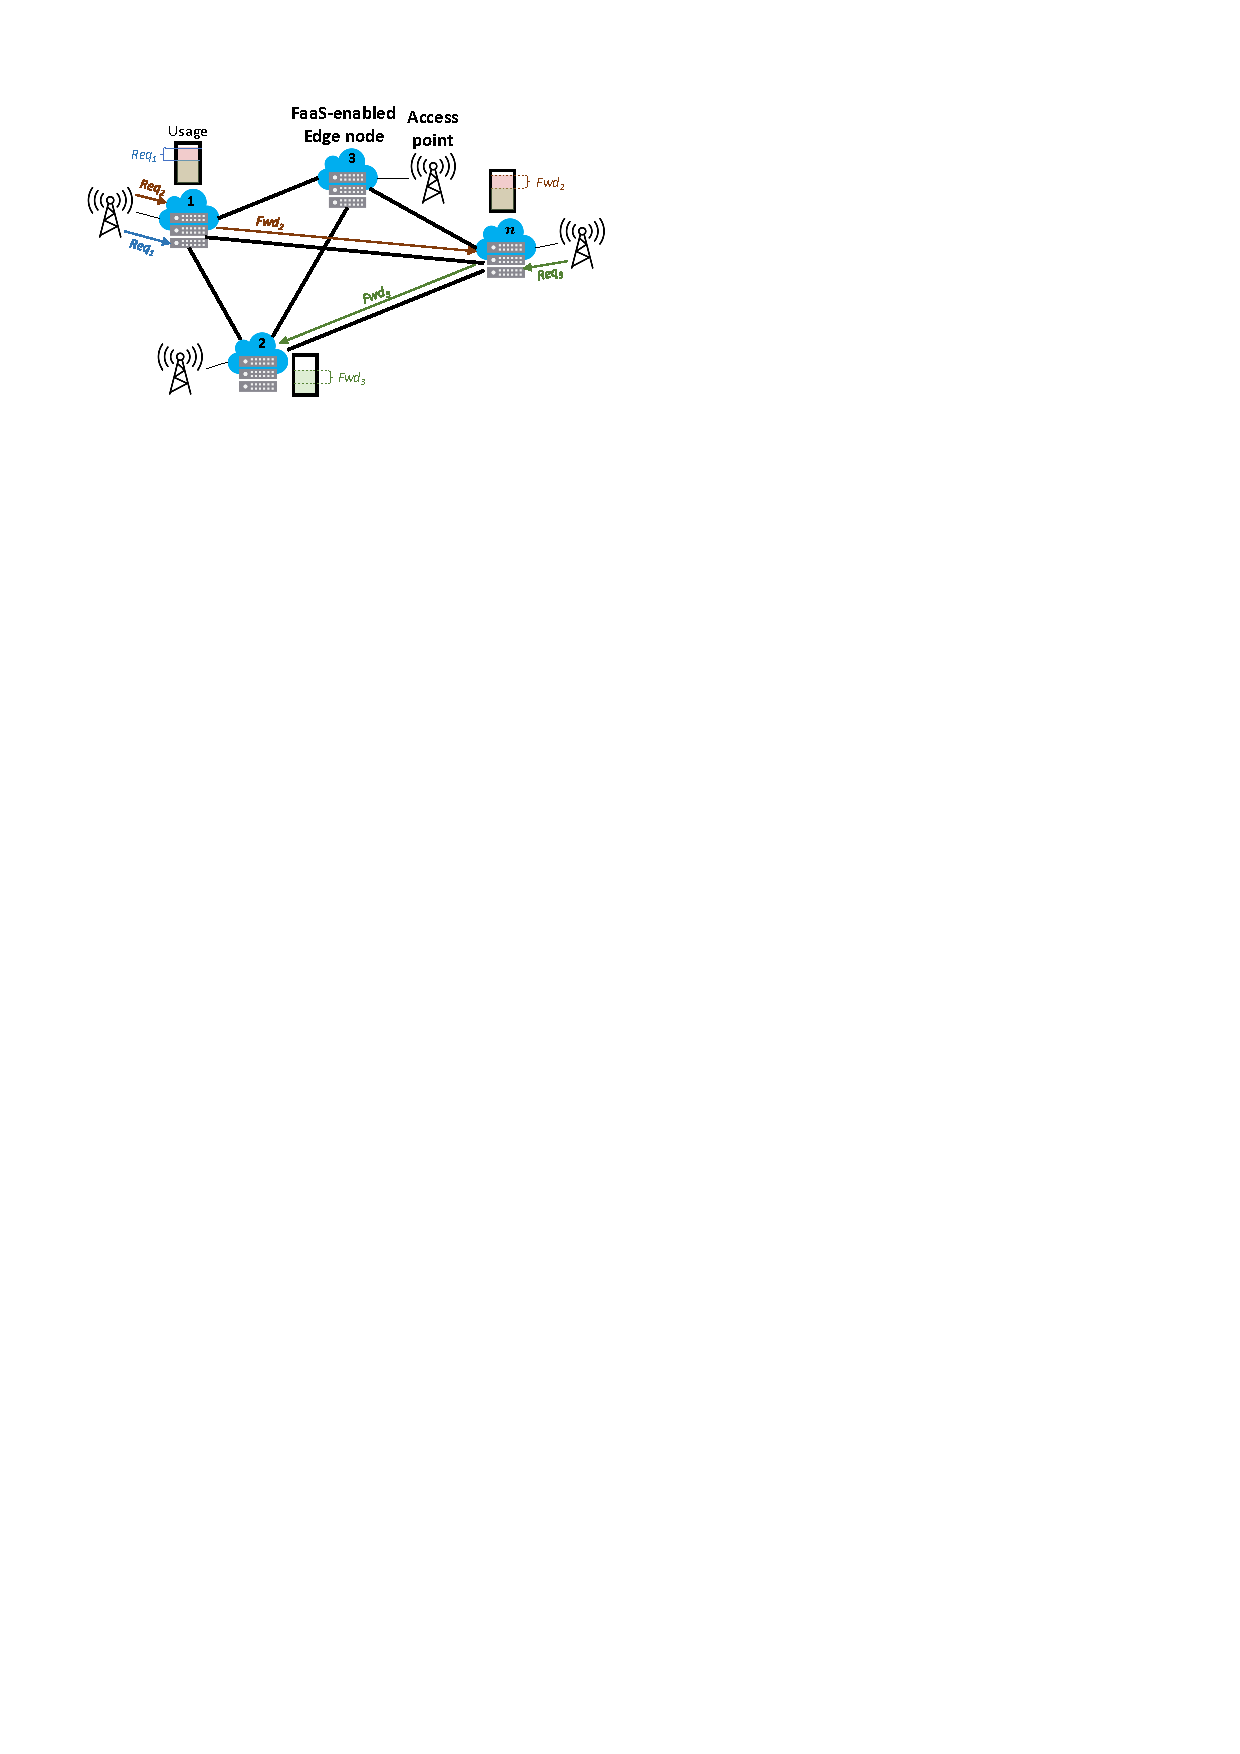
\includegraphics[width=\columnwidth]{assets/2/dfaas_scenario.pdf}
    \caption[Scenario di riferimento di DFaaS]{Scenario di riferimento di DFaaS in \cite{Ciavotta2021}}
    \label{fig:dfaas_scenario}
\end{figure}

In ogni nodo sono presenti tre componenti: un agente, un proxy e una piattaforma FaaS. L'agente mantiene una connessione peer-to-peer con gli altri nodi, monitora lo stato del nodo locale e prevede il carico in ingresso in arrivo nel futuro. Inoltre, negozia le risorse con i nodi vicini per gestire il carico, inoltrando o accettando richieste, e configura il proxy (implementato con HAProxy\footnote{\url{https://www.haproxy.org/}}). Il proxy inoltra le richieste in arrivo e accetta le richieste inoltrate da altri nodi per passarle alla piattaforma FaaS, basata su OpenFaaS\footnote{\url{https://www.openfaas.com/}}, la quale si occupa di eseguire le funzioni corrispondenti alle richieste.

\section{Modellazione degli ambienti}

In generale, gli algoritmi RL consistono in uno o più agenti che, a ogni passo temporale, imparano automaticamente come mappare lo stato attuale in un'azione, basandosi sull'interazione con un ambiente che reagisce fornendo un segnale numerico (la \textit{ricompensa}). Questa mappatura, chiamata \textit{policy}, è aggiornata in modo iterativo bilanciando l'esplorazione, selezionando nuove azioni non ancora scelte per visitare nuovi stati potenzialmente più fruttuosi, e lo sfruttamento, usando l'esperienza accumulata per scegliere l'azione nota attualmente come migliore \cite{Sutton2018}. Un modello di RL è, in breve, caratterizzato dalla definizione dello spazio delle osservazioni (elementi dell'ambiente osservabili dagli agenti in ogni istante), dello spazio delle azioni (come un agente può agire sull'ambiente) e dalla funzione di ricompensa.

Nel problema affrontato in questa tesi, gli agenti decidono come distribuire le richieste in ingresso in base allo stato, composto dal numero di richieste in ingresso, stato della coda e informazioni relative alle richieste inoltrate al passo precedente, codificato nelle \textit{osservazioni}, scegliendo di conseguenza un'\textit{azione} per la cui viene restituita una \textit{ricompensa} che influenza il processo decisionale. La ricompensa viene calcolata con una \textit{funzione di ricompensa}. La decisione avviene in uno spazio continuo, in cui gli agenti decidono quale percentuale di richieste in arrivo processare localmente, inoltrare a un altro agente e rifiutare per garantire una latenza ridotta, e quindi una migliore esperienza dal punto di vista dell'utente.

I tre modelli progettati, che semplificano lo scenario di riferimento DFaaS pur mantenendone le caratteristiche principali, sono raffigurati nella \Cref{fig:environments}. Differiscono, in modo incrementale, per la capacità degli agenti di inoltrare o meno le richieste in ingresso agli altri agenti. Sono di seguito definiti:

\begin{itemize}
    \item \textbf{Ambiente simmetrico senza inoltro}: ogni agente è indipendente dagli altri e lo spazio delle azioni è limitato al processamento locale e al rifiuto delle richieste. Etichettato come ``BASE'' nelle figure.

    \item \textbf{Ambiente asimmetrico}: gli agenti sono divisi in due gruppi disgiunti, uno in grado di inoltrare le richieste agli altri nodi e uno che non può inoltrare. Etichettato come ``ASYM'' nelle figure.

    \item \textbf{Ambiente simmetrico con inoltro}: ogni agente può processare localmente, inoltrare agli altri agenti o rifiutare le richieste in ingresso. Etichettato come ``SYM'' nelle figure.
\end{itemize}

Ogni agente osserva la coda locale del nodo corrispettivo, di capacità uguale per tutti gli agenti e che si svuota a ogni passo. L'ambiente è di tipo episodico di 288 passi, ogni passo rappresenta 5 minuti che coprono l'arco di una giornata di 24 ore. La scelta di considerare 5 minuti è motivata dal desiderio di dare tempo agli agenti, nel corrispettivo scenario reale, di reagire con maggiore robustezza ai cambiamenti nel carico su un periodo più esteso dei secondi o del singolo minuto.

\begin{figure}
    \centering

    \begin{subfigure}{\columnwidth}
        \centering
        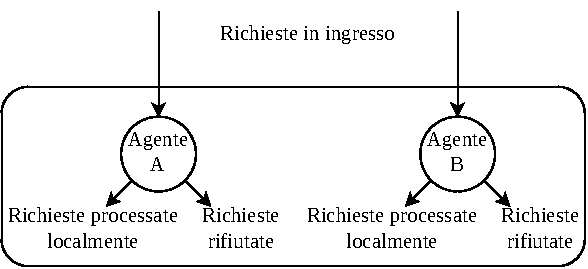
\includegraphics[width=\linewidth]{assets/4/1_sym_no_fw.pdf}
        \caption{Ambiente ``BASE''.}
    \end{subfigure}
    
    \begin{subfigure}{\columnwidth}
        \centering
        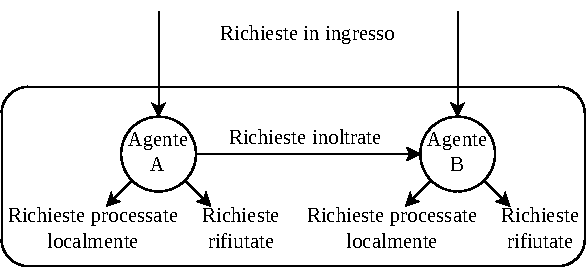
\includegraphics[width=\linewidth]{assets/4/2_asym.pdf}
        \caption{Ambiente ``ASYM''.}
    \end{subfigure}

    \begin{subfigure}{\columnwidth}
        \centering
        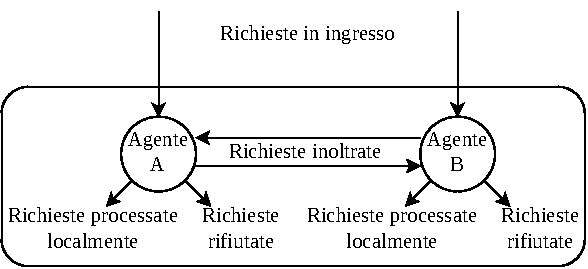
\includegraphics[width=\linewidth]{assets/4/3_sym_fw.pdf}
        \caption{Ambiente ``SYM''.}
    \end{subfigure}
    
    \caption{I tre ambienti progettati con due agenti ciascuno.}
    \label{fig:environments}
\end{figure}

Sono state definite \textbf{due funzioni di ricompensa} per gli agenti, in base alla capacità dell'agente di inoltrare o meno. Per entrambe il codominio è un numero reale in $[0, 1]$ e indica la qualità dell'azione scelta dall'agente in base allo stato dell'ambiente. L'obiettivo di entrambe è di incentivare il processamento delle richieste rispetto al rifiuto, dando priorità alla coda locale e poi all'inoltro, in caso di capacità residua esaurita, e infine di rifiutare le richieste se non è possibile né inoltrare né processare localmente.

\section{Algoritmo PPO}

È stato scelto di utilizzare l'algoritmo Proximal Policy Optimization (PPO) \cite{Schulman2017} per addestrare gli agenti, dal momento che supporta spazi di azione continui ed è risultato avere migliori prestazioni rispetto ad algoritmi simili nel contesto di singolo agente \cite{Petriglia2024}. PPO è un algoritmo basato sul Deep Reinforcement Learning (DRL), un campo del RL che combina il RL con il Deep Learning, utilizzando le reti neurali per approssimare la funzione che valuta il valore atteso di scegliere una specifica azione in uno specifico stato in base alla policy dell'agente.

% non dell'agente. L'agente vuole massimizzare la ricompensa attesa sul lungo periodo -- expected return --, e quello che viene approssimato è una funzione che valuta il valore atteso di scegliere una specifica azione in uno specifico stato

PPO è stato progettato per imparare direttamente la policy ottimale senza approssimare in modo esplicito il valore di ogni possibile azione. Questa caratteristica è importante, poiché, essendo lo spazio delle azioni continuo, effettuare una stima diretta del valore delle azioni sarebbe irrealizzabile. In aggiunta, PPO è basato sull'architettura \textit{Actor-Critic}, in cui sono presenti due reti neurali: una rete \textit{Actor} che decide in ogni stato che azione eseguire, e una rete \textit{Critic} che valuta l'azione scelta fornendo un segnale di errore utilizzato per ottimizzare le future scelte.

Nel contesto MARL sono stati sperimentati due approcci:

\begin{itemize}
    \item Fase di \textbf{addestramento ed esecuzione decentralizzata}: ogni agente viene addestrato in modo indipendente, usando solo le osservazioni locali dell'agente.

    \item Fase di \textbf{addestramento centralizzata ed esecuzione decentralizzata}: nella fase di addestramento gli agenti condividono la rete Critic, mentre la rete Actor, quella che apprende la policy, rimane indipendente. In fase di esecuzione, ogni agente ottiene una copia della rete Critic addestrata ed esegue la policy senza condividere le osservazioni.
\end{itemize}

\section{Sezione sperimentale}

L'obiettivo dell'analisi sperimentale consiste nel validare la realizzabilità di un ambiente multi-agente per la distribuzione del carico con l'algoritmo PPO, sia nella sua versione normale (``PPO'') sia nella sua versione con la rete Critic condivisa (``PPO-CC''). Nello specifico, l'analisi vuole dimostrare che, al crescere della complessità degli ambienti, permettendo quindi di inoltrare le richieste, gli agenti siano in grado di processare una maggiore percentuale delle richieste in arrivo, a fronte di carichi in ingresso di natura diversa.

\subsection{Configurazione e metodologia}

Nell'implementazione ed esecuzione degli esperimenti è stato utilizzato il framework RLlib \cite{Liang2018}, una libreria open source che implementa algoritmi di RL e strumenti per la definizione di ambienti, esecuzione e valutazione degli esperimenti in Python. I tre ambienti sono stati configurati in modo da considerare due nodi, e quindi due agenti, ognuno con capacità della coda locale  a 100. Le richieste in ingresso possono variare all'interno dell'intervallo $[0, 150]$. Sono stati progettati tre scenari di carichi in ingresso:

\begin{itemize}
    \item \textbf{Scenario reale}: carichi che consistono in tracce scelte dal dataset pubblicato in \cite{Shahrad2020}, composto da dati reali di esecuzione di funzioni FaaS nella piattaforma Microsoft Azure Functions. Le tracce sono state selezionate e ridimensionate per rispettare le dimensioni degli ambienti progettati.

    \item \textbf{Scenario sintetico sinusoidale}: carichi di tracce generate di forma sinusoidale, con l'aggiunta di un rumore proveniente da una distribuzione gaussiana per rendere meno prevedibile il traffico agli agenti. Il periodo della sinusoide cambia tre volte nell'arco di un episodio.

    \item \textbf{Scenario sintetico gaussiano}: carichi di tracce generate da una distribuzione gaussiana, con media e deviazione standard uguali ai valori estratti dalle tracce reali.
\end{itemize}

Esempi di tracce sono mostrati in \Cref{fig:input_requests_type}. In ogni episodio, i due agenti ricevono tracce diverse ma appartenenti allo stesso scenario.

La fase sperimentale è composta da due parti: la fase di addestramento, in cui ogni agente viene addestrato con PPO e PPO-CC e tutte le possibili combinazioni di scenari e tipologia di ambienti, e la fase di valutazione, in cui ogni agente viene valutato distribuendo il traffico per 50 episodi per ogni scenario. Ogni addestramento ha una durata di 500 iterazioni, e in ognuna sono eseguiti 15 episodi per un totale di \numprint{7500} episodi. Le tracce reali sono state suddivise in due insiemi, uno di addestramento e uno di valutazione. Ogni esperimento è riproducibile: in questo modo gli agenti in esperimenti diversi, ma con lo stesso scenario, sono addestrati con le stesse tracce per poter comparare le prestazioni. Avviene la stessa cosa in fase di valutazione.

\paragraph{Configurazione di PPO} La versione implementata di PPO in RLlib utilizza entrambi gli approcci PPO-Clip e PPO-Penalty, descritti in \cite{Schulman2017}, per limitare l'aggiornamento della policy ed evitare un collasso delle prestazioni. Utilizza inoltre la GPU per velocizzare l'addestramento delle reti neurali. PPO è stato configurato utilizzando gli iperparametri predefiniti in RLlib\footnote{\url{https://github.com/ray-project/ray/blob/releases/2.10.0/rllib/algorithms/ppo/ppo.py}}, derivati da \cite{Schulman2017} e ottimizzati per scenari generali. Le due reti neurali, una Actor e una Critic, sono entrambe completamente connesse con due strati nascosti da 256 nodi ciascuna e Tanh come funzione di attivazione. Il primo strato di input e l'ultimo di output sono creati automaticamente in base alle dimensioni dello spazio delle osservazioni e delle azioni.

\paragraph{Metrica di valutazione} La metrica principale che vogliamo massimizzare in ogni episodio è il \textbf{numero totale di richieste processate}. Tale metrica misura quanto un agente (o entrambi gli agenti, come nella \Cref{sec:results}) sia riuscito a distribuire in maniera ottimale il carico in ingresso. È importante osservare che il numero di richieste processabili in un episodio potrebbe essere minore del numero di richieste in ingresso: se, in un passo, i due agenti ricevono più richieste di quante la capacità complessiva delle due code locali consenta di elaborare localmente (considerando anche la possibilità di inoltro), un certo numero di richieste dovrà essere inevitabilmente rifiutato.

\subsection{Risultati}
\label{sec:results}

In questa sezione vengono presentati rapidamente i risultati degli esperimenti, mostrando nella \Cref{fig:results_requests} la percentuale di richieste processate rispetto al numero di richieste processabili per episodio, per ogni combinazione di scenario, ambiente e algoritmo. I valori mostrati sono mediati su tutte le valutazioni per un singolo esperimento e sommati per i due agenti. In generale, si osserva che tutti gli agenti imparano a processare le richieste, superando in media il 70\% delle richieste processabili.

I tre scenari sono stati progettati per avere difficoltà diversa: lo scenario gaussiano è il più semplice perché le richieste in arrivo variano intorno a un valore medio inferiore alla capacità della coda degli agenti. Ciò viene confermato nei risultati negli ambienti ASYM e SYM, mentre per BASE è vero solo usando l'algoritmo PPO-CC: in quest'ultimo caso, infatti, l'addestramento con PPO riscontra difficoltà a processare le richieste su tutti e tre gli scenari, oltre a essere poco stabile e suscettibile ai singoli carichi.

PPO-CC influisce in modo positivo nell'ambiente SYM, dove gli agenti riescono a sfruttare al meglio la rete Critic condivisa per collaborare e processare più richieste, ottenendo pertanto un risultato migliore di PPO. Ciò non vale per gli ambienti BASE e ASYM, in cui la capacità di inoltro degli agenti viene limitata. 

Si può osservare che gli agenti addestrati con tracce reali mostrano una crescita delle richieste processate all'aumentare della complessità degli ambienti. Gli agenti dell'ambiente SYM con le tracce reali ottengono infatti i risultati migliori in assoluto. Gli agenti addestrati con questo ambiente inoltre risultano più stabili.

Lo scenario sintetico sinusoidale risulta essere il più complesso da gestire: le tracce in ingresso possono essere in fase e rendere difficile il lavoro agli agenti, poiché entrambi saranno impossibilitati a processare le richieste localmente o ad inoltrarle. Un inoltro eccessivo può infatti portare a un peggioramento delle prestazioni.

\begin{figure}
    \centering

    \begin{subfigure}{\columnwidth}
        \centering
        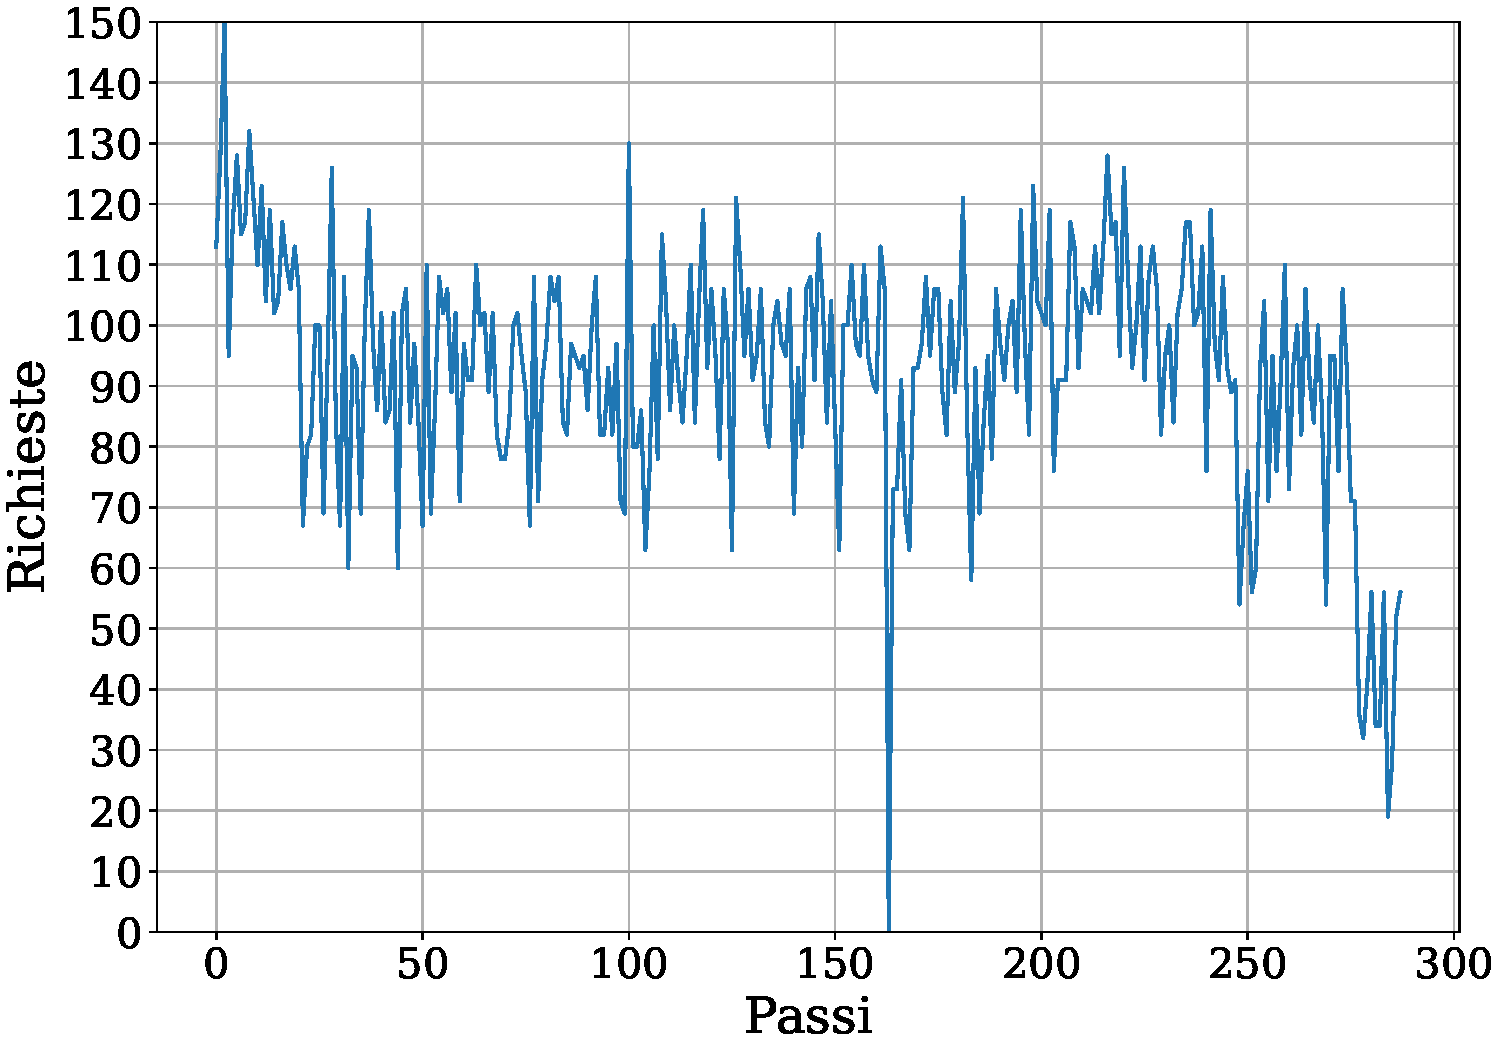
\includegraphics[width=\linewidth]{assets/5/requests_real_64425_single_agent.pdf}
        \caption{Traccia reale.}
    \end{subfigure}
    
    \begin{subfigure}{\columnwidth}
        \centering
        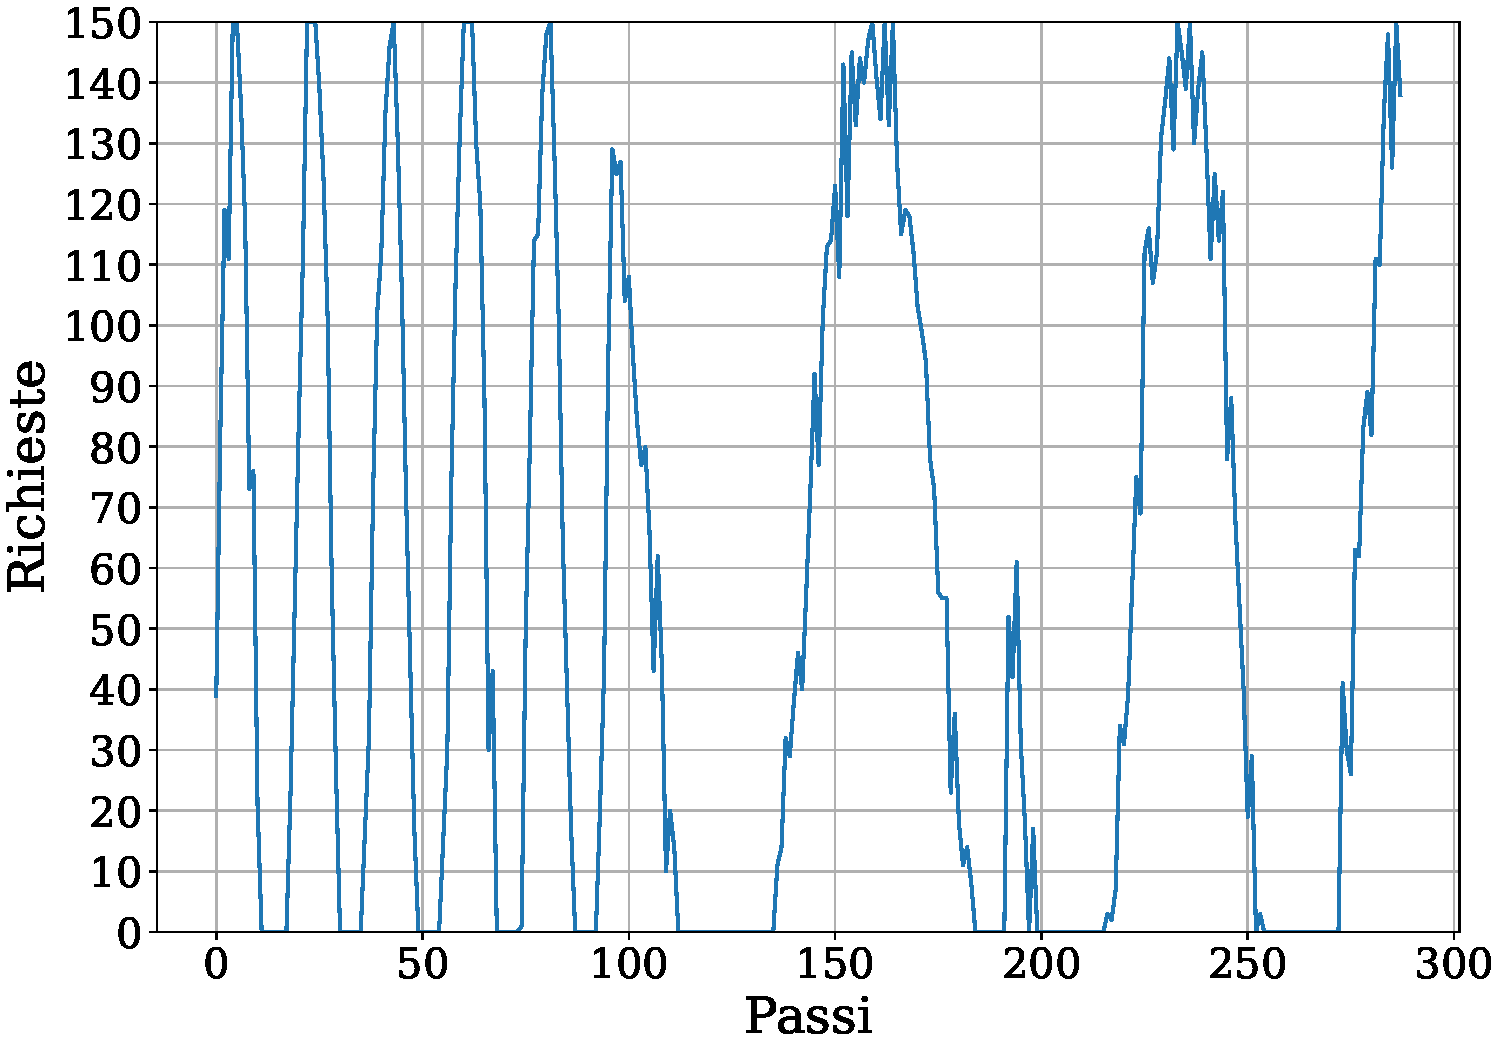
\includegraphics[width=\linewidth]{assets/5/requests_sinusoidal_64425_single_agent.pdf}
        \caption{Traccia sintetica sinusoidale.}
    \end{subfigure}
    
    \begin{subfigure}{\columnwidth}
        \centering
        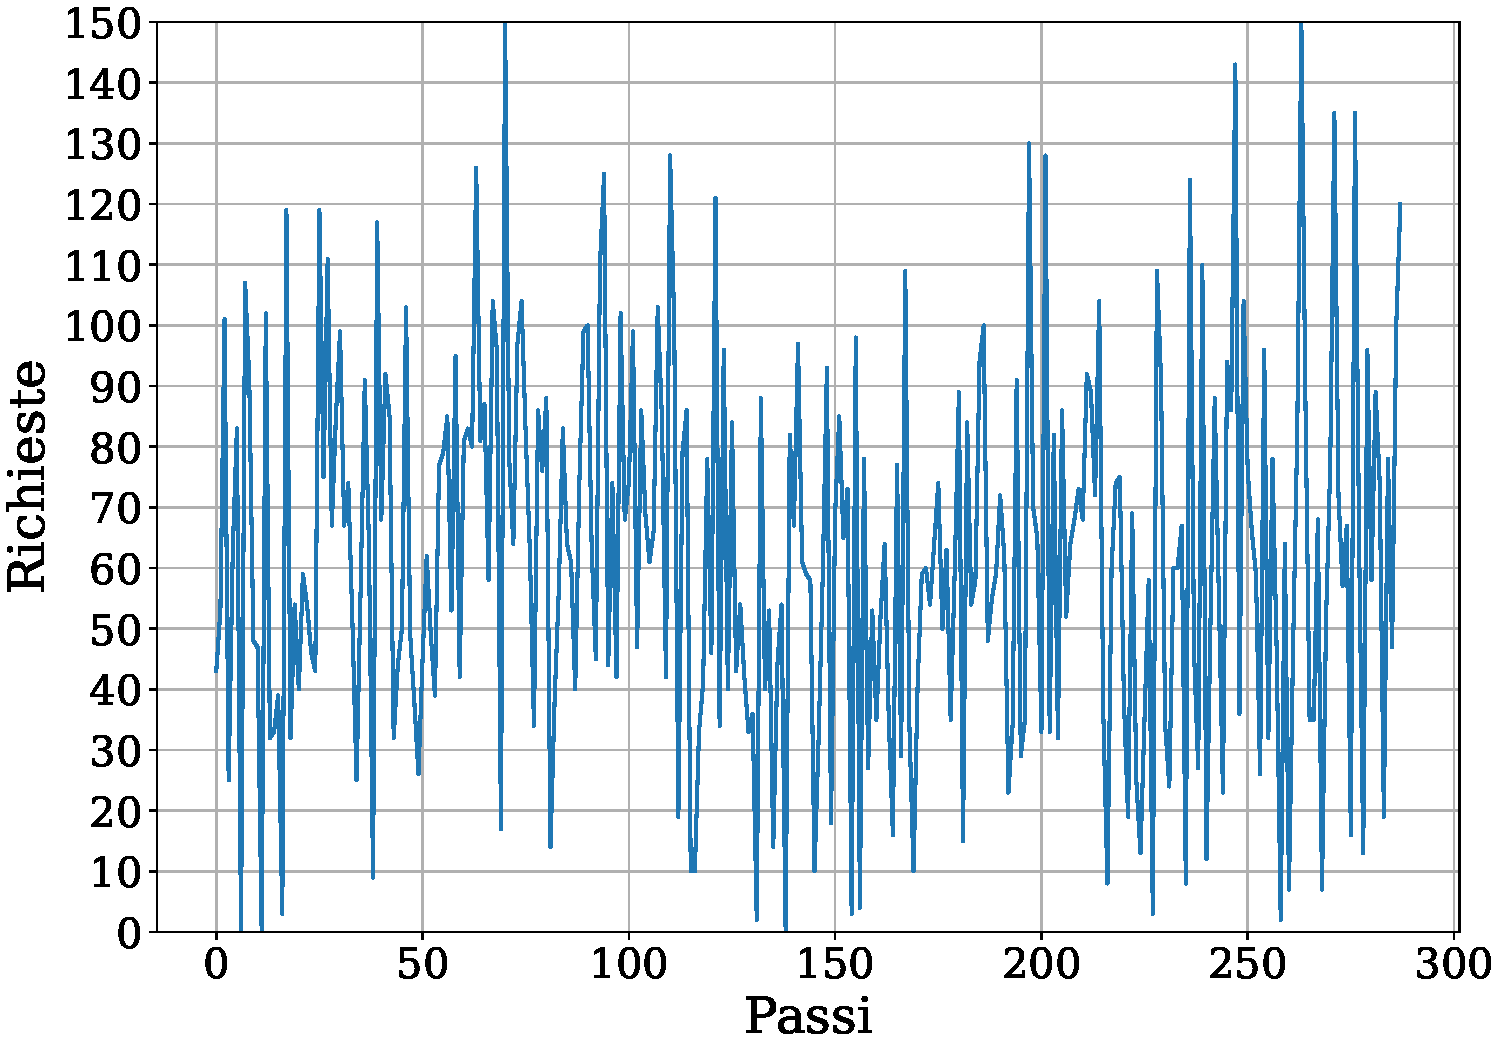
\includegraphics[width=\linewidth]{assets/5/requests_normal_64425_single_agent.pdf}
        \caption{Traccia sintetica gaussiana.}
    \end{subfigure}
    
    \caption{Esempio di tracce per le tipologie di scenario.}
    \label{fig:input_requests_type}
\end{figure}

\begin{figure}
    \centering

    \begin{subfigure}{\columnwidth}
        \centering
        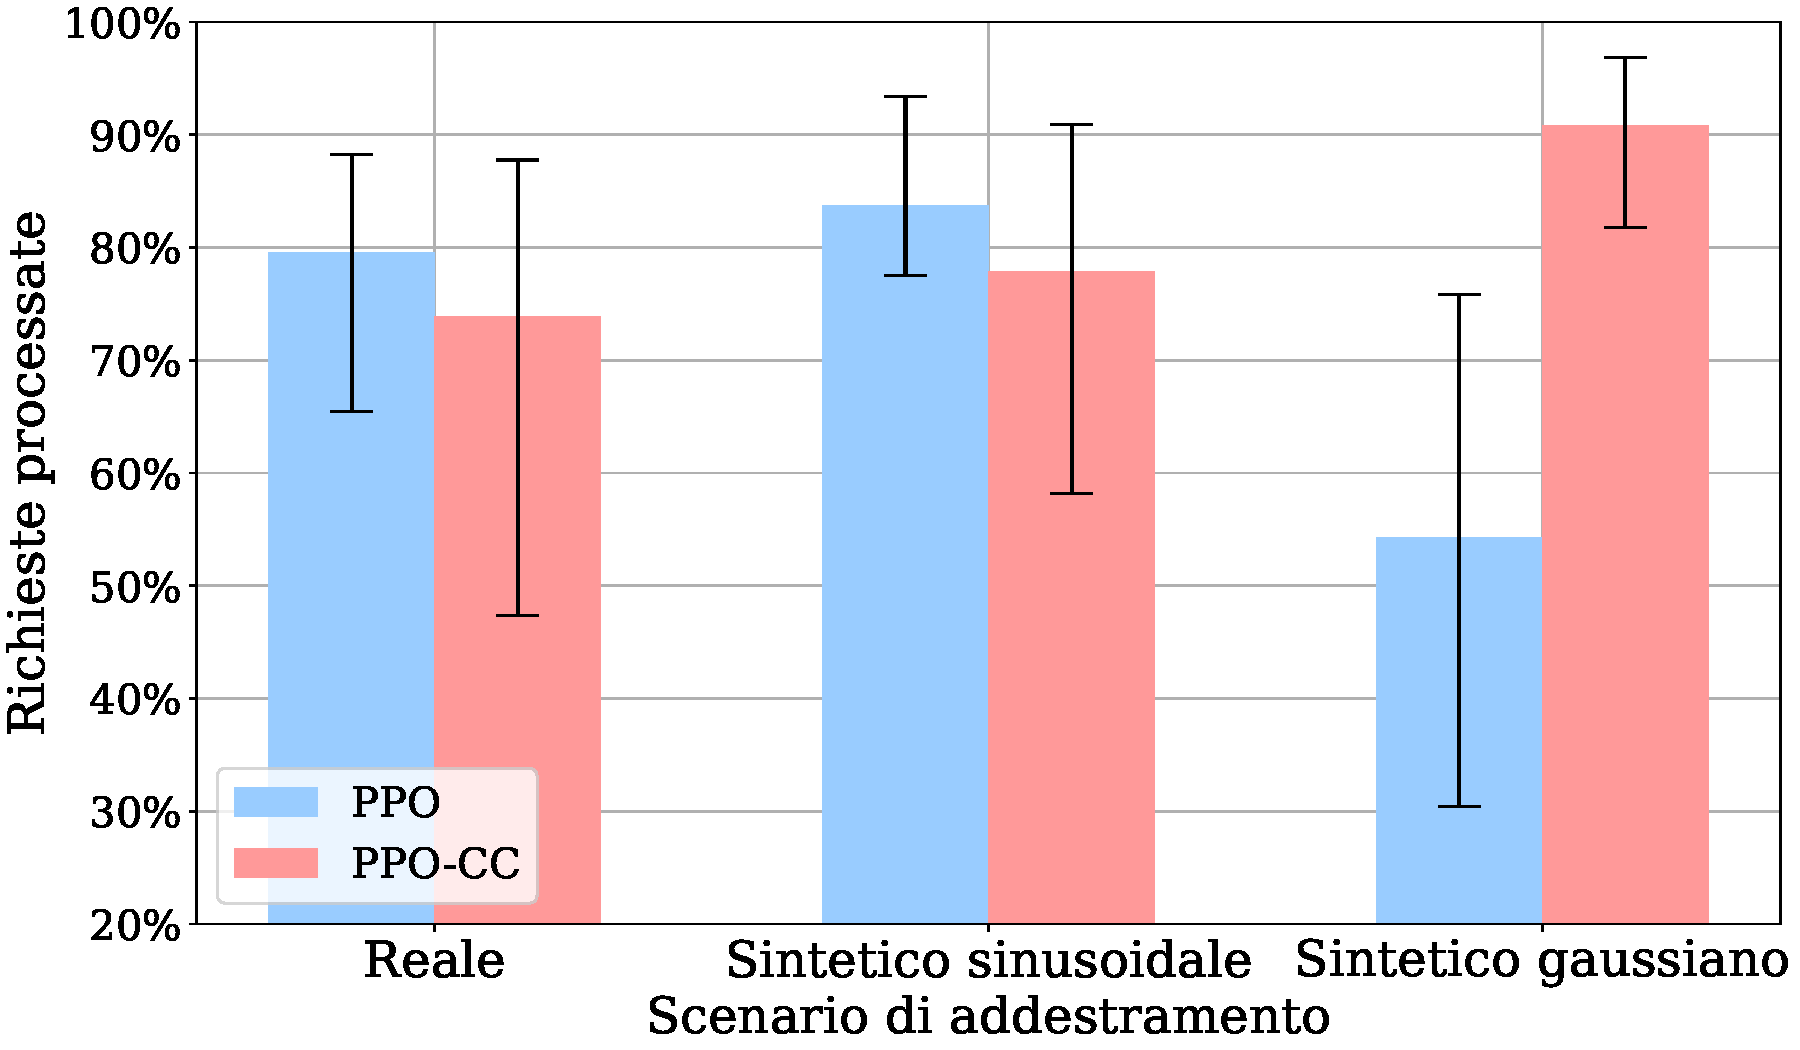
\includegraphics[width=\linewidth]{assets/5/results/eval_BASE_summary_processed_requests.pdf}
        \caption{Ambiente ``BASE''.}
    \end{subfigure}
    
    \begin{subfigure}{\columnwidth}
        \centering
        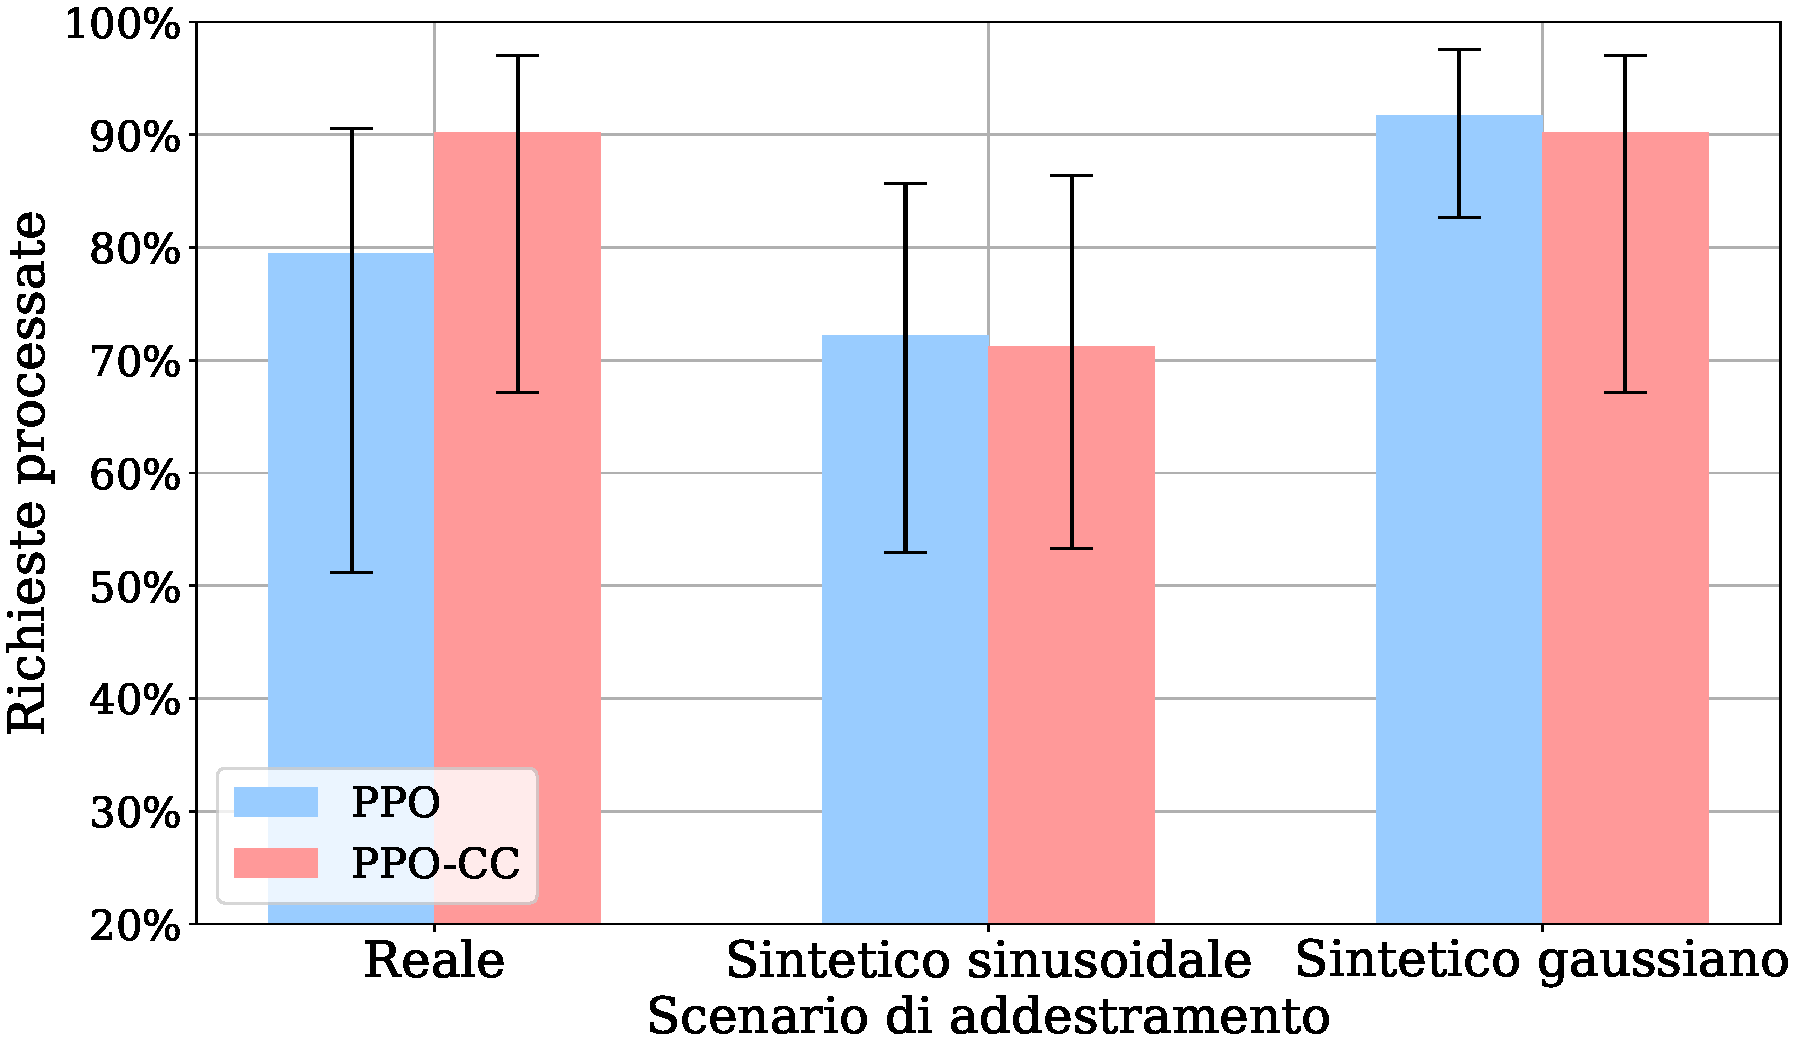
\includegraphics[width=\linewidth]{assets/5/results/eval_ASYM_summary_processed_requests.pdf}
        \caption{Ambiente ``ASYM''.}
    \end{subfigure}
    
    \begin{subfigure}{\columnwidth}
        \centering
        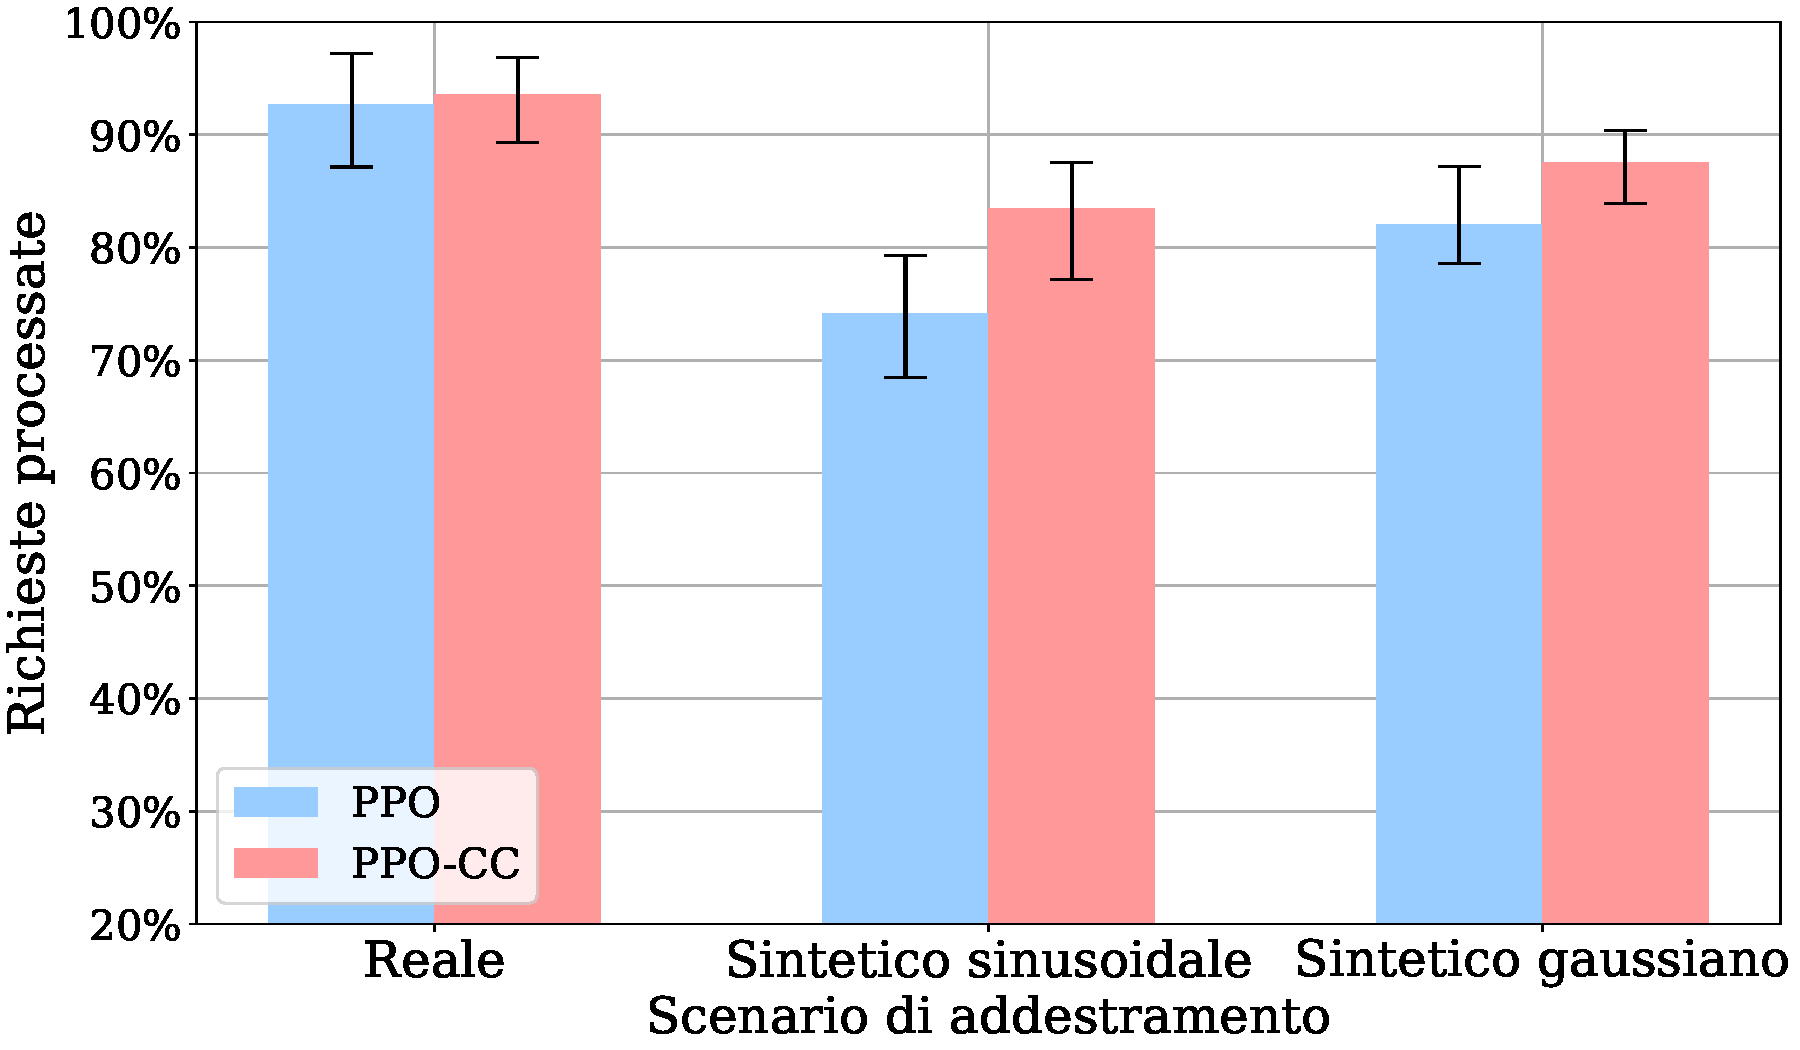
\includegraphics[width=\linewidth]{assets/5/results/eval_SYM_summary_processed_requests.pdf}
        \caption{Ambiente ``SYM''.}
    \end{subfigure}
    
    \caption{Percentuale media di richieste processate su tutte le valutazioni con valori di minimo e massimo (in nero). La percentuale è rispetto al massimo numero di richieste processabili per episodio.}
    \label{fig:results_requests}
\end{figure}

\section{Conclusione}

Questa tesi presenta lo sviluppo preliminare di un approccio basato su MARL per la distribuzione del carico in sistemi decentralizzati edge FaaS. In particolare, propone un modello semplificato del problema e utilizza un algoritmo di RL in due forme diverse, una completamente decentralizzata e una con la fase di addestramento centralizzata. I risultati mostrano che il RL, e in particolare il MARL, può essere utilizzato per affrontare questo problema, con PPO e PPO-CC che elaborano oltre il 70\% delle richieste processabili in ingresso.

Sviluppi futuri si concentreranno sulla generazione di un modello di un ambiente più complesso, che si avvicini più a un sistema DFaaS reale. Inoltre, verrà esplorato in modo più approfondito l'approccio MARL, al fine di migliorare la collaborazione e cooperazioni degli agenti.

\printbibliography[title=Riferimenti bibliografici]

\end{document}